\chapter{Background}
\label{chapter:Background}
This section summarizes the necessary background topics of the thesis.
Each topic is introduced independently, interrelation is done during synthesis of hypotheses for this thesis in chapter \ref{chapter:Hypotheses}.


\section{Relations}
This section introduces the necessary aspects of mathematical relations for this thesis.
The concept of relations is a generalization of semantic dependencies between two or more mathematical objects.
This section is based on \cite{DBLP:books/sp/SchmidtS89}.

Relations are based on set-theory. We also introduce the necessary constructs of set-theory in order to clarify terminology and notation.
A set is a collection of well distinguishable mathematical objects.
Objects in a set are called elements of the set.
A set does not contain two or more identical elements.
The notation $x \in X$ denotes that $x$ is an element of the set $X$.
The symbol $\emptyset$ denotes the \emph{empty set}, which contains no elements.
The symbol $\universe$ denotes the universal set, which contains all elements.

\begin{definition}[Inclusion]
\label{definition:Inclusion}
Let $X$ and $Y$ be a sets.
$Y$ \emph{includes} $X$ if and only if:
\begin{align}
X \subset Y 
&:\Leftrightarrow \forall x [x \in X \rightarrow x \in Y]
\Leftrightarrow \forall x [x \not\in X \vee x \in Y ]
\end{align}
Then $X$ is called \emph{subset} of $Y$ and $Y$ is called \emph{superset} of $X$.
For an arbitrary set $Z \neq \emptyset$, the statement $\emptyset \subset Z$ is always true, respectively $Z \subset \emptyset$ is always false.
\end{definition}
We also define the opposite property: $Y$ does not include $X$ if and only if:
\begin{align}
X \not\subset Y
&:\Leftrightarrow \exists x [x \in X \wedge x \not\in Y]
\end{align}

\begin{definition}[Union]
Let $X$ and $Y$ be a sets.
\begin{align}
X \cup Y &:= \{ x | x \in X \vee x \in Y \} 
\end{align}
$X \cup Y$ is called \emph{union} of $X$ and $Y$.
\end{definition}

\begin{definition}[Intersection]
Let $X$ and $Y$ be a sets.
\begin{align}
X \cap Y &:= \{ x | x \in X \wedge x \in Y \} 
\end{align}
$X \cap Y$ is called \emph{intersection} of $X$ and $Y$.
\end{definition}

\begin{definition}[Power-Set]
\label{definition:PowerSet}
Let $X$ be a set, then the \emph{power-set} of $X$ is defined as:
\begin{align}
\mathcal{P}(X) := \{ Y | Y \subset X \}
\end{align}
\end{definition}

The definition of inclusion provides an order for power-sets.
So we may compare two sets $A$ and $B$ in the sense of \emph{smaller} and \emph{larger}, i.e.:
\begin{align}
A \text{ is smaller than } B 
&\Leftrightarrow A \subset B
\\
A \text{ is larger than } B  
&\Leftrightarrow B \subset A
\\
A \text{ is the smallest subset of } B
&\Leftrightarrow \forall C \in \powersetOf{B} : A \subset C
\\
A \text{ is the largest subset of } B
&\Leftrightarrow \forall C \in \powersetOf{B} : C \subset A
\end{align}


\begin{definition}[Upper \& Lower Bound]
Let $\universe$ be a universe, $X \in \powersetOfUniverse$ be a set in the universe and $A \subset \mathcal{P}(U), A \neq \emptyset,$ non-empty subsets in the universe.
\begin{align}
X \text{ is an \emph{upper bound} for } A
&:\Leftrightarrow
\forall Y \in A : Y \subset X
\\
X \text{ is a \emph{lower bound} for } A
&:\Leftrightarrow
\forall Y \in A : X \subset Y
\end{align}
We also define:
\begin{align}
\mathbf{U}_A 
&:= \{ U \in \powersetOfUniverse | \forall Y \in A : Y \subset U \}
\\
\mathbf{L}_A
&:= \{ L \in \powersetOfUniverse | \forall Y \in A : L \subset Y \}
\end{align}
as sets of all upper/lower bounds for $A$.
\end{definition}

Because our definition of upper and lower bounds is based on power-sets, existence is guaranteed:
Given an arbitrary set $S$, the $S$ and $\emptyset$ are always elements of $\powersetOf{S}$.
For each element $Y$ of a non-empty selection $A \subset \powersetOf{S}$ of the power-set, $Y \subset S$ and $\emptyset \subset Y$ holds.
So $S$ is an upper and $\emptyset$ is a lower bound for $A$.

\begin{definition}[Supremum \& Infimum]
\label{definition:SupremumAndInfimum}
Let $\universe$ be a universe, $X \in \powersetOfUniverse$ be sets in the universe and $A \subset \powersetOfUniverse, A \neq \emptyset$ a non-empty selection of sets in the universe.
If
\begin{align}
X 
= \sup A
:= \bigcup\limits_{Y \in A} Y
&:\Leftrightarrow
X \in \mathbf{U}_A \wedge \forall U \in \mathbf{U}_A : X \subset U
\\
X
= \inf A
:= \bigcap\limits_{Y \in A} Y
&:\Leftrightarrow
X \in \mathbf{L}_A \wedge \forall L \in \mathbf{L}_A : L \subset X
\end{align}
then $X$ is called \emph{supremum}/\emph{infimum} for $A$.
\end{definition}

Existence for supremum and infimum is guaranteed, because upper and lower bounds exist as shown above.
Thus, for any non-empty selection $A \subset \powersetOf{S}$ of a power-set, $\mathbf{U}_A$ and $\mathbf{L}_A$ are not empty.
So we need to proof, that $X = \bigcup\limits_{Y \in A} Y$ respectively $X = \bigcap\limits_{Y \in A} Y$ are in fact the smallest upper and the  largest lower bound.
Or in other words:
Does another bound $X' \in \mathbf{U}_A$ respectively $X' \in \mathbf{L}_A$ exist with $X' \neq X$ and $X' \subset X$ respectively $X \subset X'$?
\begin{enumerate}
\item
Supremum:
We assume $X' \in \mathbf{U}_A$ with $X' \neq X$ and $X' \subset X$ for $X = \bigcup\limits_{Y \in A} Y$ exists, then an element $x \in X$ exists, which is not element of $X'$.
Because $X$ is the union of all sets in selection $A$, $x$ must be element of at least one of its sets.
However, then $X'$ cannot include sets containing $x$.
Thus, $X'$ cannot be an upper bound for $A$ and $X = \sup A$.

\item
Infimum:
We assume $X' \in \mathbf{L}_A$ with $X' \neq X$ and $X \subset X'$ for $X = \bigcap\limits_{Y \in A} Y$ exists, then an element $x \in X'$ exists, which is not element of $X$.
Because $X$ is the intersection of all sets in selection $A$, $x$ cannot be element of at least one of its sets.
However, then $X'$ must include sets containing $x$.
Thus, $X'$ cannot be a lower bound fo $A$ and $X = \inf A$.

\end{enumerate}
Supremum and Infimum are unique for any non-empty selection of sets in a universe and can be obtained by its union respectively its intersection.
\cite{DBLP:books/sp/SchmidtS89}

\begin{definition}[Cartesian Product]
Let $U$ be a universe and $X_n \in \mathcal{P}(U)$ sets with $ i=1...n, n \in \mathbb{N}$, then:
\begin{align}
X_1 \times ... \times X_n := \{ (x_1,..., x_n) \}
\end{align} 
is called \emph{Cartesian product}.
\end{definition}

\begin{definition}[Relation]
A relation is a subset of a Cartesian product:
\begin{align}
R \subset X_1 \times ... \times X_n 
\end{align}
The relation of only two sets is called \emph{binary relation}.
Instead of writing $(x,y) \in R$ we may also use the shorter notation $xRy$.
\end{definition}

An arbitrary relation $R \subset A \times B$ is called \emph{homogeneous} if $A = B$, otherwise it is called \emph{heterogeneous}.
However, an arbitrary relation $R \subset A \times B$ is also homogeneous in the sense of
$R \subset A \times B \subset (A \cup B) \times (A \cup B)$.
For the remainder of this section we focus on homogeneous relations unless noted otherwise.

In order to clarify our notation, when we are specifically working with relations instead of ordinary sets, we use the symbols
$\sqsubset$ for inclusion,$\not\sqsubset$ for non-inclusion, $\sqcup$ for union and $\sqcap$ for intersection, i.e.:
\begin{align}
R \sqsubset S
&:\Leftrightarrow
\forall x,y [(x,y) \in R \rightarrow (x,y) \in S]
\\
R \not\sqsubset S
&:\Leftrightarrow
\exists x,y [(x,y) \in R \wedge (x,y) \not\in S]
\\
R \sqcup S
&:=
\{ (x,y) | (x,y) \in R \vee (x,y) \in S \}
\\
R \sqcap S
&:=
\{ (x,y) | (x,y) \in R \wedge (x,y) \in S \}
\end{align}
Furthermore, we use $\relationsOver{A}$ to denote the set of all homogeneous relations in set $A$ and the symbols $\emptyRelation$ and $\allRelation$ to denote the empty relation and the universal relation:
\begin{align}
\relationsOver{A} 
&:= \{ R | R \subset A \times A \}
\\
(\emptyRelation &:= \emptyset) \subset A \times A
&\Leftrightarrow
\forall R \in \mathcal{R}(A) [ \emptyRelation \sqsubset R ]
\\
(\allRelation &:= A \times A) \subset A \times A
&\Leftrightarrow
\forall R \in \mathcal{R}(A) [ R \sqsubset \allRelation ]
\end{align}

\begin{definition}[Composition of Binary Relations]
%Let $R \subset A \times B$ and $S \subset C \times D$ be two binary relations.
%Then $S \circ R \subset A \times D$ is defined
%\begin{align}
%R \circ S = RS := \{ (a,d) \in A \times D | \exists x \in B \cap C : (a,x) \in R \wedge (x,d) \in S \}
%\end{align}
Let $R,S \in \relationsOver{A}$.
Then $R \circ S \in \relationsOver{A}$ is defined
\begin{align}
R \circ S 
= RS 
:= \{ (r,s) \in A \times A | \exists x \in A : (r,x) \in R \wedge (x,s) \in S \}
\end{align}
and called \emph{composition} or \emph{multiplication} of $R$ and $S$.
Instead of writing $R \circ S$ we also write simply $RS$.
\end{definition}
In conjunction with $\sqsubset$ composition is monotone:
\begin{align}
\forall P,Q,R \in \relationsOver{A}:
 P \sqsubset Q \rightarrow R \circ P \sqsubset R \circ Q
\\
\forall P,Q,R \in \relationsOver{A}:
 P \sqsubset Q \rightarrow P \circ R \sqsubset Q \circ R  
\end{align}
\begin{itemize}
\item
($\Rightarrow$)
Following the definition of composition, it can easily be observed, if $Q$ includes $P$, all elements of $P$ are also in $Q$:
\begin{align}
&\forall x,y: (x,y) \in R \circ P
\\&\rightarrow
\exists z : (x,z) \in R \wedge (z,y) \in P 
\overset{P \sqsubset Q}{\rightarrow}
\exists z :  (x,z) \in R \wedge (z,y) \in Q
\\&\rightarrow 
(x,y) \in R \circ Q
\end{align}
An analogous deduction can be shown for the right hand side composition of $R$.

\item
($\Leftarrow$)
The opposite direction can be proven indirectly, assuming $R \circ P \sqsubset R \circ Q$ holds, but $P \sqsubset Q$ does not:
\begin{align*}
&\forall x,y: (x,y) \in R \circ P \rightarrow (x,y) \in R \circ Q
\\&\Leftrightarrow
\exists z : (x,z) \in R \wedge (z,y) \in P \vee [(x,z) \in R \]
\overset{P \not\sqsubset Q}{\rightarrow}
\exists z : (x,z) \in R \wedge (z,y) \in P \wedge (z,y) \not\in Q
\end{align*}

\end{itemize}




\begin{definition}[Identity Relation]
The relation $\idRelation \in \relationsOver{A}$
\begin{align}
\idRelation &:= \{ (a,b) \in A \times A | a = b \} = \{ (a,a) | a \in A \} \subset A \times A
\end{align}
is called \emph{identity relation}.
\end{definition}

$(\relationsOver{A},\circ,\idRelation)$ is a monoid, i.e. for all relations in $\relationsOver{A}$ composition is associative and $\idRelation$ serves as it's identity element:
\begin{align}
&(Q \circ R) \circ S 
= Q \circ (R \circ S)
\\
&R \circ \idRelation 
= \idRelation \circ R = R
\end{align}
Also, $\emptyRelation$ serves as absorbing element for composition:
\begin{align}
R \circ \emptyRelation = \emptyRelation \circ R = \emptyRelation
\end{align}

Because $(\relationsOver{A},\circ,\idRelation)$ is a monoid, we can define exponentiation:

\begin{definition}[Exponentiation of Relations]
Let $R \in \relationsOver{A}$ and $n \in \mathbb{N}$.
\begin{align}
R^{0} &:= \idRelation
\\R^{n} &:= R \circ R^{n-1}
\end{align}
\end{definition}

Consider the following example:
\begin{align}
A &= \{a,b,c,d\}\\
R &= \{(a,b),(a,c),(c,d)\}\\
R^{0} &= \{(a,a),(b,b),(c,c),(d,d)\}\\
R^{1} &= R \circ R^{0} = R \circ \idRelation = \{(a,b),(a,c),(c,d) \}\\
R^{2} &= R \circ R^{1} = R \circ R = \{(a,d)\}\\
R^{3} &= R \circ R^{2} = \emptyRelation\\
R^{4} &= R^{5} = R^{6} = ... = R \circ \emptyRelation = \emptyRelation
\end{align}


%\begin{definition}[Properties of Relations]
%%Let $R \subset A \times A$ and $S \subset A \times B$ be homogeneous or arbitrary relations, they may satisfy one or more of the following properties:
%Let $R \in \relationsOver{A}$ it may satisfy one or more of the following properties:
%\begin{align}
%%\emph{bijective} 
%%&:\Leftrightarrow
%%\forall b \in B \exists! a \in A: (a,b) \in S
%%\\
%%\emph{function} 
%%&:\Leftrightarrow
%%\forall a \in A \exists! b \in B: (a,b) \in S
%%\\
%\emph{reflexive} 
%&:\Leftrightarrow
%\forall a \in A: (a,a) \in R
%\\
%\emph{irreflexive} 
%&:\Leftrightarrow
%\forall a \in A: (a,a) \not\in R
%\\
%\emph{transitive} 
%&:\Leftrightarrow
%\forall a,b,c \in A: (a,b) \in R \wedge (b,c) \in R \Rightarrow (a,c) \in R
%\\
%\emph{intransitive} 
%&:\Leftrightarrow
%\forall a,b,c \in A: (a,b) \in R \wedge (b,c) \in R \Rightarrow (a,c) \not\in R
%\\
%\emph{symmetric} 
%&:\Leftrightarrow
%\forall a,b \in A: (a,b) \in R \Rightarrow (b,a) \in R
%\\
%\emph{asymmetric} 
%&:\Leftrightarrow
%\forall a,b \in A: (a,b) \in R \Rightarrow (b,a) \not\in R
%\\
%\emph{antisymmetric} 
%&:\Leftrightarrow
%\forall a,b \in A: (a,b) \in R \wedge (b,a) \in R \Rightarrow a = b
%\end{align}
%\end{definition}

\begin{definition}[Reflexivity]
A relation $R \in \relationsOver{A}$ is called:
\begin{align}
\emph{reflexive} 
&:\Leftrightarrow
\forall a \in A: (a,a) \in R
\\
\emph{irreflexive} 
&:\Leftrightarrow
\forall a \in A: (a,a) \not\in R
\end{align}
\end{definition}

\begin{definition}[Reflexive Closure]
Let $R \in \relationsOver{A}$.
Then
\begin{align}
R^\circ
:= \inf \{ S | R \sqsubset S \wedge S \text{ reflexive } \}
= R \sqcup \idRelation
\end{align}
is called \emph{reflexive closure} of $R$.
\end{definition}

The reflexive closure of a homogeneous relation $R$ is the infimum or largest lower bound of the set $A = \{ S | R \sqsubset S \wedge S \text{ reflexive } \}$ containing all reflexive relations, which include $R$.
The smallest reflexive relation is $\idRelation$.
The smallest relation including $R$ is $R$ itself.
So, for an arbitrary relation $R' \in A$ the inclusions $R \sqsubset R'$, $\idRelation \sqsubset R'$ and $(R \sqcup \idRelation) \sqsubset R'$ hold.
Thus $R \sqcup \idRelation$ is a lower bound for $A$ and $(R \sqcup \idRelation) \sqsubset \inf A$ holds.
Vice versa, $R \sqcup \idRelation$ is an element of $A$ and any relation $R'' \sqsubset (R \sqcup \idRelation)$ does either not include $R$ or is not reflexive.
Thus $R \sqcup \idRelation$ is also the smallest relation in $A$ and $\inf A \sqsubset (R \sqcup \idRelation)$.
From $(R \sqcup \idRelation) \sqsubset \inf A$ and $\inf A \sqsubset (R \sqcup \idRelation)$ follows $\inf A = (R \sqcup \idRelation)$.
\cite{DBLP:books/sp/SchmidtS89}

\begin{definition}[Symmetry]
\label{definition:Symmetry}
A relation $R \in \relationsOver{A}$ is called:
\begin{align}
\emph{symmetric} 
&:\Leftrightarrow
\forall a,b \in A: (a,b) \in R \Rightarrow (b,a) \in R
\\
\emph{asymmetric} 
&:\Leftrightarrow
\forall a,b \in A: (a,b) \in R \Rightarrow (b,a) \not\in R
\\
\emph{antisymmetric} 
&:\Leftrightarrow
\forall a,b \in A: (a,b) \in R \wedge (b,a) \in R \Rightarrow a = b
\end{align}
\end{definition}

\begin{definition}[Transitivity]
A relation $R \in \relationsOver{A}$ is called:
\begin{align}
\emph{transitive} 
&:\Leftrightarrow
R^{2} \sqsubset R
\\&:\Leftrightarrow
\forall a,b,c \in A: (a,b) \in R \wedge (b,c) \in R \rightarrow (a,c) \in R
\\
\emph{intransitive} 
&:\Leftrightarrow
R^{2} \not\sqsubset R
\\&:\Leftrightarrow
\forall a,b,c \in A: (a,b) \in R \wedge (b,c) \in R \rightarrow (a,c) \not\in R
\end{align}
\end{definition}
The equivalent characterization of transitivity is $R^{2} \sqsubset R$ is easily obtained:
\begin{align}
&\forall a,b,c \in A: (a,b) \in R \wedge (b,c) \in R \Rightarrow (a,c) \in R
\\&\Leftrightarrow
\forall a,c \in A: (a,c) \in RR \rightarrow (a,c) \in R
\\&\Leftrightarrow
\forall a,c \in A: (a,c) \in R^{2} \rightarrow (a,c) \in R
\\&\Leftrightarrow
R^{2} \sqsubset R 
\end{align}
If $\mathcal{T}(A) := \{ R \in \relationsOver{A} | R^{2} \sqsubset R \}$ is the set over all transitive relations of set $A$, it's infimum $I := \inf \mathcal{T}(A)$ is also transitive.
Assuming it is not, at least one element exists, which is in $I^{2}$, but not in $I$.
Because $I$ is the infimum of $\mathcal{T}(A)$, all transitive relations $R$ must include it.
Thus the same element is in $R^{2}$, but not in $R$.
However, this is a contradiction, because $R$ is transitive and all elements in $R^{2}$ must be in $R$.
\begin{align}
\neg(I^{2} \sqsubset I)
&\Leftrightarrow
\forall x,y : \neg[(x,y) \in I^{2} \rightarrow (x,y) \in I]
\\&\Leftrightarrow
\forall x,y : (x,y) \in I^{2} \wedge (x,y) \not\in I
\\&\Leftrightarrow
\forall x,y \exists z : (x,z) \in I \wedge (z,y) \in I \wedge (x,y) \not\in I
\\&\Leftrightarrow
\forall x,y \exists z : (x,z) \in R \wedge (z,y) \in R \wedge (x,y) \not\in R
\\&\Leftrightarrow
\forall x,y : (x,y) \in R^{2} \wedge (x,y) \not\in R
\\&\Leftrightarrow
\forall x,y : \neg[(x,y) \in R^{2} \rightarrow (x,y) \in R]
\\&\Leftrightarrow
\neg(R^{2} \sqsubset R) 
\text{\lightning}
\end{align}


\begin{definition}[Transitive Closure]
Let $R \in \relationsOver{A}$ and $i \in \mathbb{N}$.
Then
\begin{align}
R^{+}
:= \inf \{ S | R \sqsubset S \wedge S \text{ transitive } \}
= \sup \{ R^{i} | i \geq 1 \}
\end{align}
%$R^{+} := R^{1} \cup R^{2} \cup R^{3} \cup ...$
is called \emph{transitive closure} of $R$.
\end{definition}

The transitive closure of a relation is the infimum or greatest lower bound of the set $A = \{ S | R \sqsubset S \wedge S \text{ transitive } \}$ containing all transitive relations, which include $R$.
Because $A$ contains only transitive relations, its infimum $I = \inf A$ is also transitive.

\begin{align*}
&PR \sqsubset QS
\\&\Leftrightarrow
\forall x,y:
(x,y) \in PR \rightarrow (x,y) \in QS
\\&\Leftrightarrow
\forall x,y \exists z:
(x,z) \in P \wedge (z,y) \in R \rightarrow (x,z) \in Q \wedge (z,y) \in S
\\&\Leftrightarrow
\forall x,y \exists z:
(x,z) \not\in P \vee (z,y) \not\in R
\vee 
[(x,z) \in Q \wedge (z,y) \in S]
\\&\Leftrightarrow
\forall x,y \exists z:
[(x,z) \not\in P \vee (z,y) \not\in R \vee (x,z) \in Q]
\wedge
[(x,z) \not\in P \vee (z,y) \not\in R \vee (z,y) \in S]
\\&\Leftrightarrow
\forall x,y \exists z:
[(z,y) \not\in R \vee [(x,z) \not\in P \vee (x,z) \in Q]]
\wedge
[(x,z) \not\in P \vee [(z,y) \not\in R \vee (z,y) \in S]]
\\&\Leftrightarrow
\forall x,y \exists z:
[(z,y) \not\in R \vee [(x,z) \in P \rightarrow (x,z) \in Q]]
\wedge
[(x,z) \not\in P \vee [(z,y) \in R \rightarrow (z,y) \in S]]
\\&\Leftrightarrow
\forall x,y \exists z:
[(z,y) \not\in R \vee P \sqsubset Q]
\wedge
[(x,z) \not\in P \vee R \sqsubset S]
\end{align*}

\begin{align*}
&PR \not\sqsubset QS
\\&\Leftrightarrow
\exists x,y : (x,y) \in PR \wedge (x,y) \not\in QS
\\&\Leftrightarrow
\exists x,y,z: [(x,z) \in P \wedge (z,y) \in R] \wedge \neg[(x,z) \in Q \wedge (z,y) \in S]
\\&\Leftrightarrow
\exists x,y,z: [(x,z) \in P \wedge (z,y) \in R] \wedge [(x,z) \not\in Q \vee (z,y) \not\in S]
\\&\Leftrightarrow
\exists x,y,z:
[(x,z) \in P \wedge (z,y) \in R \wedge (x,z) \not\in Q]
\vee
[(x,z) \in P \wedge (z,y) \in R \wedge (z,y) \not\in S]
\\&\Leftrightarrow
\exists x,y,z:
[P \not\sqsubset Q \wedge (z,y) \in R]
\vee
[(x,z) \in P \wedge R \not\sqsubset S]
\\&\Leftrightarrow
\forall x,y,z:
\neg([P \not\sqsubset Q \wedge (z,y) \in R]
\vee
[(x,z) \in P \wedge R \not\sqsubset S])
\\&\Leftrightarrow
\forall x,y,z:
[P \sqsubset Q \vee (z,y) \not\in R]
\wedge
[(x,z) \not\in P \vee R \sqsubset S]
\\&\Leftrightarrow
\forall x,y,z:
[[P \sqsubset Q \vee (z,y) \not\in R] \wedge (x,z) \not\in P ]
\vee
[[P \sqsubset Q \vee (z,y) \not\in R] \wedge R \sqsubset S]
\\&\Leftrightarrow
\forall x,y,z:
[P \sqsubset Q \wedge (x,z) \not\in P] 
\vee 
[(z,y) \not\in R \wedge (x,z) \not\in P]
\vee
[P \sqsubset Q \wedge R \sqsubset S]
\vee 
[(z,y) \not\in R \wedge R \sqsubset S]
\\&\Leftrightarrow
\forall x,y,z:
[P \sqsubset Q \wedge (x,z) \not\in P] 
\vee 
[(x,y) \not\in PR]
\vee
[P \sqsubset Q \wedge R \sqsubset S]
\vee 
[(z,y) \not\in R \wedge R \sqsubset S]
\end{align*}



\begin{definition}[Transitive-Reflexive Closure]
$R^{*} := R^{+} \cup I$
is called \textit{reflexive-transitive closure}
\end{definition}

\begin{definition}[Order Relation]
content...
\end{definition}
\section{Formal Languages \& Grammars}
\subsection{Context-Free Languages \& Grammars}
\section{Mereology}
\label{section:Mereology}
Mereology is the logical study on the semantics of parthood.
\textit{"As a formal theory, mereology is simply
an attempt to set out the general principles underlying the relationships between a whole and its constituent parts [...]"} \cite{DBLP:journals/dke/Varzi96}.
Achille C. Varzi describes a collection of formal theories, i.e. sets of distinct axioms, of mereology in \cite{DBLP:journals/dke/Varzi96}, which will be summarized in this section.

The first part of this section will just introduce the axioms of mereology.
Then, at the end of this section, we will use these axiom to build some of the theories described in \cite{DBLP:journals/dke/Varzi96}.
Note, that the terms relation, relationship and predicate may be used synonymously throughout this section.


\subsection{Parthood}
\label{subsection:Parthood}
First we define the intuitive notion of the parthood relationship:
\begin{definition}[$\partOf$]
Let $x$ and $y$ objects of interest.
We define:
\begin{align}
x \partOf y
:\Leftrightarrow
x \text{ is a constituent part of } y
\end{align}
\end{definition}
We further assume, that $\partOf$ satisfies the following properties:
\begin{align}
&\text{(P1)}
\qquad x \partOf x 
&\qquad \text{(Reflexivity)}
\\
&\text{(P2)}
\qquad x \partOf y \wedge y \partOf x \rightarrow x = y
&\qquad \text{(Antisymmetry)}
\\
&\text{(P3)}
\qquad x \partOf y \wedge y \partOf z \rightarrow x \partOf z
&\qquad \text{(Transitivity)}
\end{align}
Thus, $\partOf$ induces a partial order of things.

However, since the reflexive parthood may be to week for some cases, we also define a stricter, irreflexive parthood relationship as follows:
\begin{align}
x \properPartOf y
:\Leftrightarrow
x \partOf y \wedge \neg(y \partOf x)
\end{align}
Proper parthood induces a strict partial order of things.

In addition to the relationships above we introduce the following predicates in order to provide a more concise notation:
\begin{align}
x \overlaps y
&:\Leftrightarrow
\exists z : z \partOf x \wedge z \partOf y
&\qquad \text{(Overlap)}
\\
x \underlaps y
&:\Leftrightarrow
\exists z : x \partOf z \wedge y \partOf z
&\qquad \text{(Underlap)}
\end{align}
Overlap models situations, where two things share at least on distinct part.
Underlap models situations, where two things belong to the same distinct whole.

\subsection{Supplementation}
\label{subsection:Supplementation}
The fourth axiom, which can be assumed in an universe described by means of mereology, is the supplementation axiom.
It models the effects of situations more precisely, where one thing is not part of another.
Namely, if this is the case, a third thing may exist, which is part of the former but not part of the latter.
\begin{align}
&\text{(P4)}
\qquad
\neg(x \partOf y) \rightarrow \exists z (z \partOf x \wedge \neg(z \overlaps y))
\end{align}
The supplementation axiom reads: If a thing $x$ is not part of another thing $y$, then at least one part of $x$ does not share further parts with $y$.
Figure \ref{fig:SupplementaitonAxiomExample} exemplifies the supplementation axiom.

\begin{figure}[h!]
\begin{center}
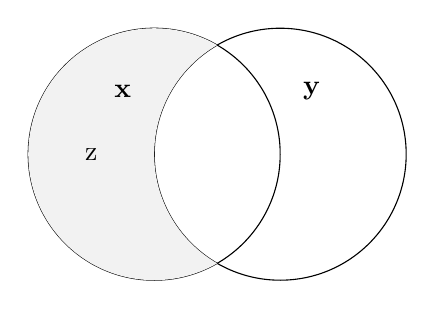
\begin{tikzpicture}[scale=0.8]
\draw(1,1)circle(2 and 2);
\draw(3,1)circle(2 and 2);
\scope
\clip (-1,-1) rectangle (3,3)
	  (3,1) circle (2 and 2);
\fill[gray!10] (1,1) circle (2 and 2);
\endscope
\draw(0.5,2)node{\textbf{x}};
\draw(3.5,2)node{\textbf{y}};
\draw(0,1)node{z};
\end{tikzpicture}
\end{center}
{
\scriptsize 
This Venn-style diagram exemplifies the supplementation axiom:
$x$ is not part of $y$.
Thus, $x$ contains a part $z$ (emphasized as gray area), which shares no further parts with $y$
}
\caption{Example for the Supplementation Axiom}
\label{fig:SupplementaitonAxiomExample}
\end{figure}

%\usetikzlibrary{calc}
%\begin{tikzpicture}[scale=0.8]
%\draw(4,3)circle(5 and 3)node(A){Text A};
%\draw(8,6)circle(5 and 3)node(B){Text B};
%\draw(10,2.5)circle(5 and 3)node(C){Text C};
%\begin{scope}
%\clip(4,3)circle(5 and 3);
%\clip(8,6)circle(5 and 3);
%\clip(10,2.5)circle(5 and 3);
%\filldraw[yellow!80](0,0)rectangle(10,10);
%\end{scope}
%\node at ($0.33*(A)+0.33*(B)+0.33*(C)$){Text M};
%\end{tikzpicture}

\ToDo{add paragraph explaining "strong" and "weak" supplementation}

One can also observe from figure \ref{fig:SupplementaitonAxiomExample}, that the supplementation axiom can be interpreted as analogue to set-theoretic difference.

\subsection{Sum, Product \& Difference}
\label{subsection:Sum}
\subsubsection{Sum}
\begin{align}
&\text{(P5)}
\quad
&\begin{split}
&x \underlaps y 
\\&\rightarrow
\exists z \forall w (x \overlaps z \leftrightarrow (w \overlaps x \vee w \overlaps y))
\end{split}
\end{align}

\begin{align}
z = x + y
:\Leftrightarrow
\forall w (x \overlaps z \leftrightarrow (w \overlaps x \vee w \overlaps y))
\end{align}

\subsubsection{Product}
\begin{align}
&\text{(P6)}
\quad
&\begin{split}
&x \overlaps y 
\\&\rightarrow
\exists z \forall w (x \partOf z \leftrightarrow (w \partOf x \wedge w \partOf y))
\end{split}
\end{align}

\begin{align}
z = x \cdot y
:\Leftrightarrow
\forall w (x \partOf z \leftrightarrow (w \partOf x \wedge w \partOf y))
\end{align}

\subsubsection{Difference}
\begin{align}
&\text{(P7)}
\quad
&\begin{split}
&\exists z (z \partOf x \wedge \neg(z \overlaps y))
\\&\rightarrow
\exists z \forall w (x \partOf z \leftrightarrow (w \partOf x \wedge \neg(w \overlaps y)))
\end{split}
\end{align}

\begin{align}
z = x - y
:\Leftrightarrow
\forall w (x \partOf z \leftrightarrow (w \partOf x \wedge \neg(w \overlaps y)))
\end{align}

\subsection{Universal Top \& Bottom}
\label{subsection:UniversalTopAndBottom}

\subsection{Mereology Theories}
\label{subsection:MereologyTheories}

\section{Traceability}
\cite{Winkler:2010:STR:1861285.1861287}
\cite{DBLP:books/daglib/p/GotelCHZEGDAMM12}
%\lipsum[1]
TBD.
\subsection{Traceability Relationship}
\subsection{Traceability Link}
\subsection{Traceability Recovery}
\subsection{Traceability Exploration}

\section{Megamodeling}
%\lipsum[1]
TBD.

\subsection{\megal}
\subsubsection{\megalxtext}

\section{Ontologies}
%\lipsum[1]
TBD.



\section{Program Analysis}
%\lipsum[1]
TBD.

\section{XML Data Binding}
%\lipsum[1]
TBD.


\subsection{Java Architecture for XML Binding (JAXB)}

\section{Object Relational Mapping}
%\lipsum[1]
TBD.



\subsection{Java Persistence API (JPA)}

\subsection{Hibernate}



\section{Another Tool For Language Recognition (ANTLR)}

